\documentclass[
11pt, paper=a4,  listof=totocnumbered, % lists are also included in table of contents
numbers=noendperiod, % Don't add a period at the end of a chapter number
]{scrreprt}
    \usepackage{chngcntr}
    \counterwithout{footnote}{chapter}
    \counterwithout{figure}{chapter}
    \counterwithout{table}{chapter}
    

\usepackage{listings}
%%%%%%%%%%%%%%%%%%%%%%%%%%%%%%%%%%%%%%%%%%%%%%%%%%%%%%%%%%%%%%%%%%%%%%%%%%%%%%%%
%%%%%%%%%%%%%%%%%%%%%%%%%%%%%% Bibliography  %%%%%%%%%%%%%%%%%%%%%%%%%%%%%%%%%%%

% get custom bibliography style working without prepending [brackets]
\usepackage[backend=biber,sortcites, style=apa]{biblatex}    %
\nocite{*}
\addbibresource{biblio.bib}

% linebreaks in bibliography urls
% \usepackage{url}
% \usepackage{breakurl}
% \def\UrlBreaks{\do\/\do-}							% add a breakpoint at - and /

%\setcounter{biburlnumpenalty}{1000}  				% add a breakpoint after all numbers
%\setcounter{biburlucpenalty}{1000}					% add a breakpoint after all uppercase letters
%\setcounter{biburllcpenalty}{1000}   				% add a breakpoint after all lowercase letters

%\usepackage{nabtib}
%\setcitestyle{aysep={}} % remove comma as delimiter 

% breaks line at hyphens (resolves formatting issues in bibliography)
%\usepackage[hyphens]{url}
\usepackage{txfonts} % Use a Times-new-roman open-source clone
% if you insist on Arial... then uncomment the following
%\usepackage{helvet}
\renewcommand{\familydefault}{\sfdefault}
\usepackage{caption}
\usepackage{float}
\setkomafont{chapter}{\Large} 
\setkomafont{section}{\large}
\setkomafont{subsection}{\large} 
\usepackage[left=2cm,right=2cm,top=2cm,bottom=2cm]{geometry} % margins
\addtolength{\footskip}{-0.7cm}% foot larger by 0,7 cm  (Raises the page number)


\usepackage[onehalfspacing]{setspace} % line space 1,5

\setlength{\parindent}{6pt} % Indent at start of paragraphs  6pt

\usepackage[utf8]{inputenc} %UTF-8 to encode many characters => for many characters, you can just input the character and avoid a macro

\usepackage[english]{babel} % english hyphenations
%\usepackage[T1]{fontenc} %wichtig für Trennung von Wörtern mit Umlauten
\usepackage{microtype} % align margins

\usepackage{graphicx} % import graphics
\usepackage{placeins}% places the graphics within text

% Abbreviation's directory
% printonlyused - only if used
% withpage - the first occurrence's page number is listed too
\usepackage[withpage]{acronym}

\usepackage[hidelinks]{hyperref} %https://tex.stackexchange.com/questions/823/remove-ugly-borders-around-clickable-cross-references-and-hyperlinks

\lstset{
	language=Python,								% default language
	numbers=left,								% line number position, alternative: none
	stepnumber=1,								 
	numbersep=6pt,								% distance between line number and code
	numberstyle=\fontsize{9pt}{9pt}\ttfamily,	% line number style
	breaklines=true,							% break lines if necessary
	breakautoindent=true,						% indent after line break
	postbreak=\space,							% break at space
	tabsize=4,									% tab size
	showspaces=false,							% do not show spaces in code
	showstringspaces=false,						% do not show spaces in strings
	extendedchars=true,							% use Latin1
	captionpos=b,								% caption position
	backgroundcolor=\color{lightGrey}, 			% background color
	xleftmargin=0pt,								
	xrightmargin=0pt,							
	frame=leftline,								% draw frame ar left side only
	framerule=1.1pt,							% frame width
	frameround=ffff,							% round corners: f = not rounded | t = rounded
	rulecolor=\color{lightBlue},				% frame color
	framesep=1.5pt,								% distance between line number and border 
	fillcolor=\color{lightGrey},
	basicstyle=\ttfamily\footnotesize\color{darkGrey},	
	keywordstyle=\color{magenta}\bfseries,
	identifierstyle=,
	commentstyle=\color{lightBlue},
	stringstyle=\color{darkBlue}
}

\lstloadlanguages{bash, C, C++, HTML, Java, PHP, Python, SQL}

% change heading above listings to \ListOfListingsTitle
\renewcommand{\lstlistlistingname}{\ListOfListingsTitle}

% Group list of listings by chapter
\let\Chapter\chapter
\def\chapter{\addtocontents{lol}{\protect\addvspace{10pt}}\Chapter}


\begin{document}

\include{001-Titlepage}

\renewcommand{\thechapter}{\Roman{chapter}}

\pagestyle{plain}

\pagenumbering{Roman} %the intro is counted with roman numbers
\setcounter{page}{2} %starting with page 2 (page 1 is the titel)

% --- too detailed for a seminar but otherwise useful
%\include{002-BlockingNotice}
%\include{003-Acknowledgements}
%\include{004-Abstract}

\tableofcontents %table of contents
\listoffigures %List of figures
\listoftables %list of tables

% Abbreviations list
\renewcommand\refname{Abbreviations} \chapter{Abbreviations}
% The abbreviations list should contain all abbreviations that are not common-knowledge.
\begin{acronym}[NMWC] % the longest abbreviation here (for layout)
    \setlength {\itemsep}{-\parsep} % geringerer Zeilenabstand   
    \acro{MLE}{Maximum Likelihood Estimate}
    \acro{cdf}{cummulative density function}
    \acro{pdf}{probability density function}
%    \acro{CPU}{Central Processing Unit}
\end{acronym}

% Acronyms should be made hyperreffed the first time they appear in text with
% \ac{CI}  

\renewcommand{\thechapter}{\arabic{chapter}} %Count chapters with arabic numbers and not roman numbers
\setcounter{chapter}{0} %Reset chapter counter
\pagenumbering{arabic}

%\chapter{Introduction}
\chapter{Answer to Workbook Question}

\section{Question One}

a) There are two variables X and Y. The realization of a sample of size 20 is given below (where X is the 
first variable and Y is the second):

\begin{table}[!h]
\small
\centering
\begin{tabular}{|l|c|r|}
\hline
X & Y \\
\hline
-8.504 & -25.44\\
02.371 & 6.51\\ 
2.176 & 288.73\\ 
0.627 & -421.32\\ 
-8.429 & 5.46\\ 
2.759 & 476.25\\ 
3.268 & 4.14\\ 
-9.362 & -366.79\\ 
6.364 & 92.37\\ 
3.569 & 612.29\\ 
6.969 & -511.51\\ 
-0.466 & 268.67\\ 
4.102 & -350.29\\ 
-8.282 & 234.35\\ 
0.509 & 185.54\\ 
-0.442 & -217.03\\ 
-3.841 & -107.11\\ 
7.938 & 367.32\\ 
-1.062 & -1019.37\\ 
-3.655 & -338.54\\
\hline
\end{tabular}
\caption{Table of X \& Y values}
\label{example:table}
\end{table}
% The table is numbered \ref{example:table}.

You are to sketch an appropriate plot that displays the values of these  points. Now calculate the sample covariance as well as the sample's expectations and variances of X and Y.\\
b) If a ball is thrown with a random angle $\theta \in  (0, 360]$ (in degrees) and a random radius $r \in (0,1]$ (in meters) both independent and uniform. Calculate the density of the variable X and Y (the cartesian coordinates of the point at angle $\theta$ and radius r as well as their expectation and variance.

\subsection{Answer to Q1(a)}
We will display the graphic in R using a scatter diagram because the random variables X and Y are suitable for a scatter plot.

% \begin{figure}[h]
% \centering
% 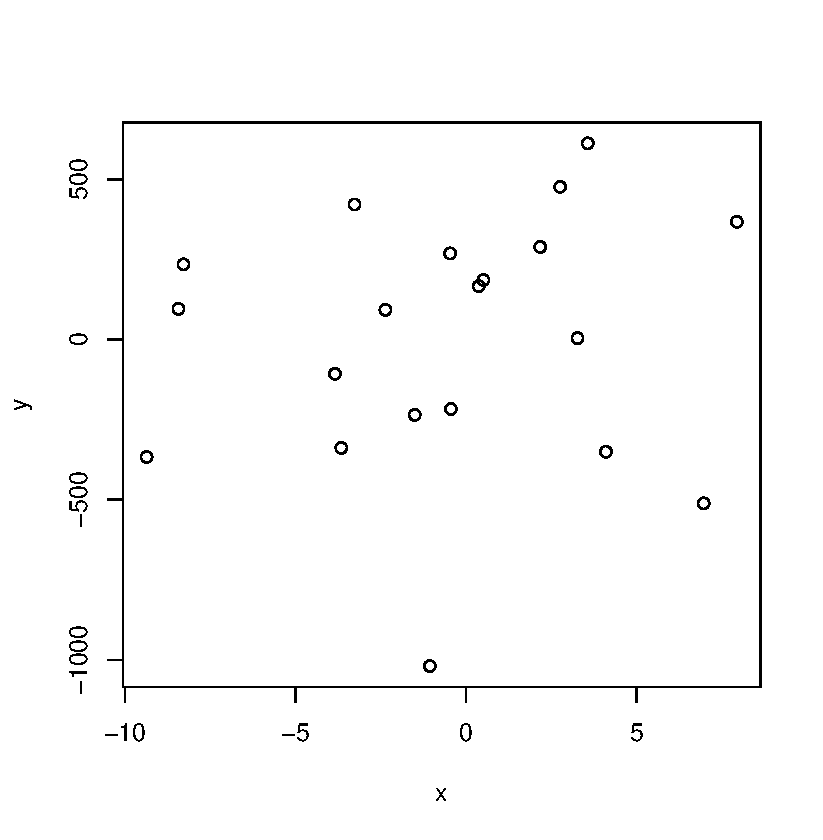
\includegraphics[width=8cm]{pics/Rplot2a.pdf}
% \caption{A graph of Probability density function for Question 2b.}
% \label{fig:2b}
% \end{figure}
% \FloatBarrier

The code for the generation of this graphic plot is (Using R):
\begin{verbatim}
x = c(-1.504, 0.371, 2.176, -3.627, -8.429, 2.759, 3.268,
-9.362, -2.364, 3.569, 6.969, -0.466, 4.102, -8.282, 0.509, 
-0.422, -3.841, 7.938, -1.062, -3.655)

y = c(-235.44, 166.51, 288.73, -421.32, 95.46, 476.25,
4.14,-366.79, 92.37, 612.29, -511.51, 268.67, -350.29, 234.35,
185.54, -217.03, -107.11, 367.32, -1019.37, -338.54)

plot(y ~ x )
\end{verbatim}

\begin{figure}[h]
\centering
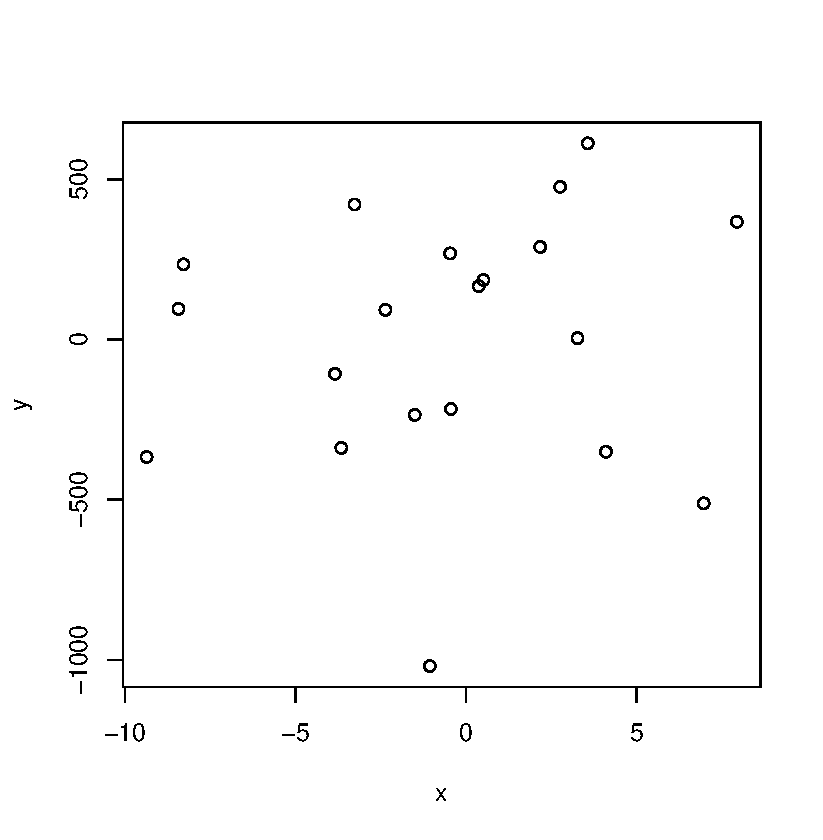
\includegraphics[width=8cm]{pics/Rplot2a.pdf}
\caption{A graph of Probability density function for Question 2b.}
\label{fig:1c}
\end{figure}
\FloatBarrier

\begin{verbatim}
abc = data.frame(x, y)
summary(abc)
\end{verbatim}

\begin{table}[!h]
\small
\centering
\begin{tabular}{|l|c|r|}
\hline
 X & Y \\
\hline    
 Min.   :-9.3620 &  Min.   :-1019.37  \\
 1st Qu.:-3.6340 &  1st Qu.: -341.48  \\
 Median :-0.4440 &  Median :   48.26  \\
 Mean   :-0.5676 &  Mean   :  -38.79  \\
 3rd Qu.: 2.8862 &  3rd Qu.:  242.93  \\
 Max.   : 7.9380 &  Max.   :  612.29  \\
\hline
\end{tabular}
\caption{Table of summary of X \& Y values}
\label{example:table}
\end{table}

Thus,
\begin{equation} \mu = \frac{\Sigma x_i}{n} \label{q2a1} \end{equation}

$$ \mu_x = \frac{-11.37}{20} = -0.5686 $$
$$ \mu_y = \frac{-775.77}{20} = -38.79 $$

And,
\begin{equation} variance = \frac{\Sigma (x_i - \mu_x)^2}{n-1} \label{q2a1} \end{equation}
$$ variance, \sigma_x = \frac{436.04}{19} = 22.95 $$
$$ variance, \sigma_y = \frac{2960947.5}{19} = 155839.3 $$

We can calculate the covariance in R \parencite[281]{Tilman:RBK}or by using equation 2.5.2 in \parencite[126]{Hogg:ITM} thus:

\begin{equation}  Cov(X,Y) = E(XY) - {\mu}_x{\mu}_y \label{q2a1} \end{equation}

Therefore,

$$ Cov(X,Y) = 381.01 - (-38.7)(-0.5686) $$
$$ Cov(X,Y) = 359.0 $$


\subsection{Answer to Q1(b)} 
From equation 2.1.5 in \cite{Hogg:ITM}, the joint \ac{cdf} of the random vector $(\theta, r)$ of space {(0,360),(0,1)}:

\begin{equation} F_{X,Y} = \int_{-\infty}^{x}\int_{-\infty}^{y}f_{X,Y}(x,y)dxdy \label{q2b} \end{equation}

And the marginal PDF's are:
$$ f(\theta) = \frac{1}{2\pi}, \theta \in [0, 2\pi) $$
$$ f(r) = 1, r \in [0, 1) $$
And we can obtain the PDF for r and $\theta$ respectively,
$$ f(\theta,r) = \frac{1}{2\pi}, r \in [0, 1), \theta \in [0, 2\pi) $$
We can invoke the polar to  coordinates conversion for use here,
\begin{equation} x = rcos\theta, y = rsin\theta, r^2 = \sqrt{x^2 + y^2}, \theta = \arctan{\frac{y}{x}} \label{q2b} \end{equation}

We would obtain our Jacobian function and substitute into this expression:
\begin{equation} f_(R,\Phi)(r,\phi) = f_(X,Y)(g^{-1}(x,y)).|J_g^{-1}(x,y)| \label{q3a1}\end{equation}

\renewcommand\arraystretch{2}

$$\left(\begin{array}{lllll}
r \\
\phi \\ 
\end{array} \right) = g\left(\begin{array}{lllll}
x \\
y \\ 
\end{array} \right) =  \left(\begin{array}{lllll}
\sqrt{x^2 + y^2} \\
\arctan{\frac{y}{x}}
\end{array} \right)
\to D{g^{-1}}(x,y)=
 \left(\begin{array}{lllll}
\frac{\partial \sqrt{x^2+y^2}}{\partial x}       & \frac{\partial \sqrt{x^2+y^2}}{\partial y} \\
\frac{\partial \arctan\frac{y}{x}}{\partial x}       & \frac{\partial \arctan\frac{y}{x}}{\partial y}\\
\end{array} \right) \to J = \sqrt{x^2 + y^2} $$
\renewcommand\arraystretch{1}

Which yields the joint pdf:
$$ f_{x,y}(x,y) = \frac{1}{2\pi \cdot \sqrt{x^2+y^2}} $$
and marginal PDF,
$$ f_x(x) = \frac{1}{2\pi} \int_{0}^{\sqrt{1-x^2}} \frac{1}{\sqrt{{x^2+y^2}}}dy = \frac{1}{4\pi}(log(\sqrt{1-x^2}+1) - log(1-\sqrt{1 - x^2})) = 0, x \in [0,1)  $$

$$ f_y(y) = \frac{1}{2\pi} \int_{0}^{\sqrt{1-y^2}} \frac{1}{\sqrt{{x^2+y^2}}}dx = \frac{1}{4\pi}(log(\sqrt{1-y^2}+1) - log(1-\sqrt{1 - y^2})) = \frac{3}{2\pi} , y \in [0,1)  $$

And expectation of x yields,
$$ E(X) = \int_{-\infty}^{\infty}xf_x(x,y)dy $$
But more precisely, we can utilize the formula for uniform distribution since the pdfs for x and y are both uniform distributions. Hence,

$$ E(X) = \frac{a+b}{2} = \frac{0+1}{2} = 0.5 $$
$$ E(X) = \frac{a+b}{2} = \frac{0+1}{2} = 0.5 $$

and the variance for x and y,

$$ E(X) = \frac{(b - a)^2}{12} = \frac{(1-0)^2}{12} = 0.0833 $$
$$ E(Y) = \frac{(b - a)^2}{12} = \frac{(1-0)^2}{12} = 0.0833 $$

%\chapter{Conclusion}


\appendix

% ---- Bibliography ----
%	
\printbibliography[heading=bibintoc]

%\chapter{Annexes (optional)}

(with a list of them)



%\chapter{Glossary (optional)}

%\include{070-Pledge}

\end{document}
